% Moved from Section 4 of the long version (sections/s4_bistability.tex) to keep the article at standard length.
% Text copied verbatim; only references are adapted (M- = main article; no prefix = Supplementary Material).

\subsection{Simulation protocols: full statement}\label{supp:std-bistab-prot}

All runs use the simulator of Section~\ref{app:simulator}, the gains of Section~\ref{M-sec:feasibility} ($\mathcal G=[0,1500]$) and, unless stated otherwise, the clipped command. In the \emph{step entry} the full depth and immersion act from $t=0$, starting from rest with zero history. In the \emph{face entry} the tool advances into a workpiece face normal to the feed and reaches full engagement after 40 revolutions. In the \emph{feed ramp} the feed per tooth rises linearly from zero to $f_z$ over ten revolutions. The depth limit of an entry was found on a ladder of depths up to $1.05\alim$, refined by bisection (Section~\ref{supp:bistab-prot}), each run being judged over the 300 revolutions after the entry.
% src: src/tdsim.c (opt[1]-opt[3]: ramp_f, f0, edge), src/tdsim.py (entry_revs), src/c1_unsafe_zone.py (ENTRIES, LADDER), src/tdboundary.py (boundary, classify: rtol 3e-3, NREV 300); README §11.2

In the kick protocol the cut was settled by a face entry, and at revolution 100 a velocity increment $\Delta v$, the \emph{kick}, was added to $\dot x$ at one of 16 phases $\theta$ per tooth period; the 300 revolutions after it were classified. The \emph{critical kick} $\Delta v^*(\theta)$ is the smallest kick that ends in chatter; as the outcome is not monotone in $\Delta v$ (a large kick throws the tool out of the cut), it was found by an upward search up to \SI{3}{\metre\per\second} (Section~\ref{supp:bistab-prot}). The lower edge of the \emph{unsafe band}, in the sense of the unsafe zones of milling \citep{dombovari2015bistable,dombovari2019experimental}, was mapped every \SI{20}{\rpm} (126 speeds) as the smallest depth at which one of seven kicks from \SI{3}{\milli\metre\per\second} to \SI{3}{\metre\per\second} ends in chatter. The checks of these protocols asked for in the literature on bistable zones (kick timing, window length, number of phases, holes in the band) are summarised in Section~\ref{supp:std-bistab-checks}.
% src: src/c1_unsafe_zone.py (KICK_REV = 100, WINDOW = 300, N_PHASE = 16, DV_GRID, N_BISECT = 6, BAND_STEP = 20, BAND_DV, BAND_PHASES = 2, BAND_BISECT = 6, _critical_kick, _band_low)

As a kick or an entry transient can throw the tool out of the cut for many passes, the chip is cut against the deepest earlier pass at the same angle [Eq.~\eqref{eq:surf}] \citep{tlusty1981basic}, a full memory without which clipped chatter can grow spuriously beyond \SI{1}{\centi\metre} (Section~\ref{app:simulator}; Section~\ref{supp:bistab-prot}); only the off-axis runs of C3 (Section~\ref{M-sec:cert-c3}) used the last four passes (Section~\ref{app:lmi}). A run whose displacement exceeds \SI{1}{\centi\metre}, 200 feeds, is stopped and counted as chatter: such an excursion is a failure of the cut, whatever the model, far outside its validity, would do afterwards. Runs are classified by the criterion D1 of Section~\ref{app:simulator}, which biases step-entry boundaries near $\alim$ high: by \SIrange{0.05}{1.5}{\percent} where long runs were used to check it, by at least \SI{4.4}{\percent} at \SI{2000}{\rpm}, near the forced resonance, where the boundary reaches the top of the depth ladder, and, judging from the unclipped step-entry limits, which should lie at $\alim$, by up to about \SI{3}{\percent} at 2040--\SI{2480}{\rpm}. It does not bias kick-based limits or clipped limits well below $\alim$.
% src: README §11.2; verification/tdsim/check9_full_memory.json (bounded clipped chatter 0.43-0.59 mm with full memory and brute force; 1050 rpm, 0.9 a_lim diverges with both; nreg 4: 2 of 4 diverge, 0.554 vs 0.435 mm); src/tdboundary.py; verification/tdsim/check8_onset_long_runs.json (bias 0.05-1.47 %), check10_forced_resonance_long_runs.json (up to 4.4 %)

\subsection{The same cut, two outcomes: step entry and mechanism}\label{supp:std-bistab-two}

At \SI{2500}{\rpm} with $g=1500$ ($\alim=\SI{17.24}{\milli\metre}$) and $a=\SI{15}{\milli\metre}$, the step entry ends in clipped chatter of about \SI{0.43}{\milli\metre}, whereas the face entry settles on the forced orbit with a command of about \SI{5}{\volt}. Figure~\ref{M-fig:two} shows the settled cut at $0.9\alim$, kicked just below and just above the critical kick of that phase, \SI{7.29}{\milli\metre\per\second}: after the smaller kick the motion returns to the forced orbit although the command still reaches the clip, after the larger one it grows into clipped chatter. The forced orbit and clipped chatter therefore coexist, and in this linear-force model, at kicks of this size, it is the saturation that makes them coexist: without the clip, chatter required kicks at least 50 times larger (Fig.~\ref{M-fig:basin}; Section~\ref{supp:std-bistab-basin}). The mechanism is a loss of effective gain (Section~\ref{M-sec:bistab-df}): once the chatter component, added to $b(t)$, reaches $\Vmax$, the clip passes on only part of the feedback, and the growing chatter saturates the command further.
% src: README §11.3; verification/tdsim/check9_full_memory.json (2500 rpm, 15 mm, step entry, full memory: max |x| = 0.435 mm); paper/figures/figure_numbers.json (fig03: 0.9 a_lim = 15.51 mm, kicks 7.0/7.6 mm/s at phase 0, critical kick 7.29 mm/s); results/c1_basin.npz (2500 rpm, 0.9 a_lim, clipped: phase 0 7.288 mm/s); closed form of Eq. (xp) gives b_max = 5.37 V at 15 mm (cross-check of README "about 5 V"); ratio 50: results/c1_basin.npz (smallest ratio of unclipped to clipped minimum kick, 52.1)

\subsection{Entry limits and unsafe band: further results}\label{supp:std-bistab-map}

With the step entry the ratio of the clipped limit to $\alim$ has a median of 0.910 and a minimum of 0.736 (\SI{2460}{\rpm}), and it is below $0.97\alim$ at 157 of 251 speeds (Fig.~\ref{M-fig:map}). The face entry reaches at least $0.985\alim$ at every speed, and the feed ramp falls below $0.97\alim$ only at \SI{2000}{\rpm} ($0.957\alim$). Where the step entry binds, the better of the face entry and the feed ramp gains \SI{2.5}{\milli\metre} on average and up to \SI{4.7}{\milli\metre} (\SI{1980}{\rpm}). Without the clip the step-entry limit sits at the linear limit (median ratio 1.01; Section~\ref{supp:bistab-map}).
% src: results/c1_map.npz, results/c1_summary.json (map: step_clip, edge_clip, feed_clip, step_free, soft_minus_step_mean_mm 2.51); results/c1_map.npz recomputed: largest gain of max(face, feed ramp) over the step entry where it binds 4.741 mm at 1980 rpm (19.02 vs 23.76 mm; 4.24 mm at 2500 rpm, 13.00 vs 17.25 mm); results/c1_map.npz recomputed: a_step_free/a_lim > 1.015 at 75 speeds (1.0165-1.050); a_edge_clip and a_feed_clip = 1.05 a_lim at 500, 540, 670, 720, 1000, 1080 rpm, a_step_clip at 500, 550, 670, 1000 rpm (seven speeds in all); at the other 245 speeds a_edge_clip mean 18.200 mm, a_lim mean 18.206 mm; results/feas_g1500.npz (at_bound: 157) vs results/c1_map.npz (a_step_clip < 0.97 a_lim: 157), 110 in common; verification/tdsim/check10_forced_resonance_long_runs.json

The lower edge of the unsafe band was found at 109 of the 126 speeds, at 0.21--$0.98\alim$ (median 0.46), and always above the uncontrolled limit, at no less than $1.08\alim(0)$. That the clip cannot create chatter below $\alim(0)$ is suggested by a describing-function argument, as the clip can only lower the effective gain, and is shown for the averaged model up to $(1-10^{-3})\,a_{\mathrm{circ}}$, where $a_{\mathrm{circ}}$ has a median over the speeds of $0.967\,\alim(0)$, in Section~\ref{M-sec:cert-global} (frequency condition proved by interval arithmetic, unclipped forced orbit checked on a dense depth grid). Above $\alim(0)$ a bounded basin is expected, since the uncontrolled cut is exponentially unstable there and no bounded input can stabilise it globally \citep{hu2001book}; what the simulations add is the size of the basin and its dependence on depth, speed and entry. No band was found at 17 speeds, most of them where the gain is small (Section~\ref{supp:bistab-map}). The edge rests on kicks of up to \SI{3}{\metre\per\second}, far beyond the validity of the model, and the bisection assumes that the band has no holes in depth; a scan of the depth at nine speeds confirms the edge at all of them but finds a hole at one (Section~\ref{supp:std-bistab-checks}). The step entry exposes only the top of the band, where the entry transient exceeds the basin.
% src: results/c1_band.npz, results/c1_summary.json (band: found 109/126, ratio 0.21/0.46/0.98, over_alim0_min 1.08, none_at_rpm, g_where_none); README §11.4

\subsection{Entry limits at gains up to \SI{3000}{\volt\second\per\metre}}\label{supp:std-bistab-gain}

At 1090 and \SI{2500}{\rpm} the entry limits were also computed for $g$ up to \SI{3000}{\volt\second\per\metre}. With the step entry the clipped limit nearly stops rising above about \SIrange{1500}{1650}{\volt\second\per\metre}, at about 19.8 and \SI{13.2}{\milli\metre}, while $\alim$ reaches 41.8 and \SI{40.0}{\milli\metre} at $g=3000$; at large gains the depth is limited by the basin, which the entry transient exceeds, not by the gain (Section~\ref{supp:bistab-df}).
% src: results/c1_gainplane.npz (a_step_clip, a_edge_clip, a_lim, orbit_peak_V), results/c1_summary.json (gainplane: step_clip_plateau_mm 19.78 and 13.19, a_lim_at_3000 41.82 and 40.03, orbit_saturates_from_g 3000 and 1650); README §11.6, §13.6; results/table3_main.csv (2500 rpm: a_prop_td 6.37 mm at the reproduced gain 535.6 V s/m; a_clip3000_td 13.23 mm), table3_clip_gain_sweep.csv; a_step_clip of c1_gainplane.npz rises monotonically with g at both speeds; README §5.5

\subsection{Basin of the forced orbit: values, scales and the unclipped cut}\label{supp:std-bistab-basin}

Figure~\ref{M-fig:basin} and Table~\ref{tab:basin} give the critical kick at 1090, 1420, 2500 and \SI{2870}{\rpm} with $g=1500$, at twelve depths from 0.15 to $0.98\alim$ with the clip and at four without it. With the clip the basin is finite from 0.25--$0.80\alim$ onwards and narrows towards the limit. To give the kick a physical scale, its impulse $m\Delta v^*$ is compared with the mean cutting impulse of one tooth period, $\bar F_yT$ of Eq.~\eqref{M-eq:impulse}, where $\bar F_y$ is the mean static force normal to the feed. At $0.98\alim$ the critical kick of the worst phase carries \SIrange{2.4}{10.8}{\percent} of this impulse; as an equivalent displacement $\Delta v^*/\omega_n$ it is 2.9--\SI{13}{\micro\metre}, against a forced vibration of about \SI{4}{\micro\metre} amplitude at \SI{2500}{\rpm} and $0.9\alim$ (Fig.~\ref{M-fig:two}) and a feed of \SI{50}{\micro\metre}. Kicks of at most \SI{10}{\milli\metre\per\second} (\SI{12}{\micro\metre}) end in chatter only from 0.90--$0.95\alim$ upwards, if at all (Section~\ref{supp:bistab-basin}). Over the 16 phases the critical kick varies by at most \SI{24}{\percent}, so the basin is a property of the cut rather than of the timing of the disturbance.
% src: results/c1_basin.npz (dv, frac, vmax, tooth_impulse, mass), results/c1_summary.json (basin: first_finite_frac, impulse_098_pct, impulse_098_min_pct, phase_spread_098, phase_spread_max); src/c1_unsafe_zone.py (run_basin: tooth impulse); verification/paper/revision_runs.json (stored.kick_displacement_098: worst-phase dv at 0.98 a_lim 10.88, 5.04, 2.34, 8.12 mm/s = 13.4, 6.2, 2.9, 10.0 um at omega_n = 2 pi 129.3 rad/s, 1090/1420/2500/2870 rpm; recomputed from results/c1_basin.npz); results/c1_basin.npz recomputed: smallest depth with worst-phase dv <= 10 mm/s: 0.95, 0.90, 0.95 a_lim at 1420, 2500, 2870 rpm, none at 1090; <= 30 mm/s: 0.40, 0.80, 0.40, 0.50 a_lim at 1090, 1420, 2500, 2870 rpm; 10 mm/s / omega_n = 12.3 um; paper/figures/figure_numbers.json (fig03 orbit_x_um -26.0 to -18.6, i.e. 3.7 um amplitude)

\begin{table}[!tbp]
  \centering
  \caption{Critical kick $\Delta v^*$ of the clipped cut ($g=\SI{1500}{\volt\second\per\metre}$, $\lvert V\rvert\le\SI{9}{\volt}$): median over 16 phases and, in parentheses, the worst phase. The last column gives $m\Delta v^*$ as a percentage of the cutting impulse $\bar F_yT$ of Eq.~\eqref{M-eq:impulse}. Basin finite from: the smallest of the 12 depths at which some kick of at most \SI{3}{\metre\per\second} ends in chatter.}
  \label{tab:basin}
  \begin{tabular}{@{}rcccc@{}}
    \toprule
    Speed & Basin finite & \multicolumn{2}{c}{$\Delta v^*$ (\si{\milli\metre\per\second})} & $m\Delta v^*/(\bar F_yT)$ (\si{\percent})\\
    \cmidrule(lr){3-4}
    (rpm) & from $a/a_{\lim}$ & $a=0.9a_{\lim}$ & $a=0.98a_{\lim}$ & $a=0.98a_{\lim}$\\
    \midrule
    1090 & 0.25 & 15.3 (15.1) & 11.5 (10.9) & 4.3 (4.0)\\
    1420 & 0.80 & 13.7 (12.5) & 5.3 (5.0)   & 3.0 (2.9)\\
    2500 & 0.40 & 8.3 (7.2)   & 2.5 (2.3)   & 2.6 (2.4)\\
    2870 & 0.50 & 11.8 (11.5) & 8.7 (8.1)   & 11.5 (10.8)\\
    \bottomrule
  \end{tabular}
\end{table}
% src: results/c1_basin.npz; results/c1_summary.json (basin); README §11.5

Without the clip, no kick up to \SI{3}{\metre\per\second} ended in chatter at 13 of the 16 tested points; at the other three only kicks of 0.78--\SI{3}{\metre\per\second} in one phase did, presumably by the loss of contact that makes milling without an actuator bistable \citep{dombovari2015bistable}; whether that chatter is bounded was not checked. In this linear-force model the clip thus shrinks the basin by a factor of 52--701 where the unclipped cut also chatters after a kick, and creates the finite-amplitude instability, on this range of kicks, at nine further points (Section~\ref{supp:bistab-basin}).
% src: results/c1_basin.npz (vmax = 0 rows; ratios of the smallest unclipped to the smallest clipped kick: 52.1, 275.7, 700.9; lower bounds 3 m/s / clipped minimum: 69.7-594.9); README §11.5

\subsection{What lies beyond the basin: attractors}\label{supp:std-bistab-attr}

The classifier shows that the basin is bounded, not where a trajectory that leaves it goes. At the 29 points of Fig.~\ref{M-fig:basin} where the basin is finite, the settled cut was therefore kicked at the worst phase with 2, 2.5 and 3 times the critical kick and followed for 2000 revolutions with the full surface memory. All 87 runs ended in bounded, stationary chatter (root mean square of $x$ and of $V$ within \SI{10}{\percent} between the second and the last quarter of the run), which differs by less than \SI{0.09}{\percent} between the three kicks; none exceeded \SI{1}{\centi\metre} and none returned to the forced orbit. This chatter keeps the command on the clip for 89--\SI{99}{\percent} of the time, at 133--\SI{153}{\hertz}, with a peak-to-peak displacement of 0.08--\SI{2.0}{\milli\metre}, 1.6 to 40 times the feed per tooth, so that the tool leaves the cut periodically, which bounds the amplitude \citep{tlusty1981basic}. At these points the clipped cut is bistable in the strict sense: the forced orbit coexists with a bounded chatter attractor (Fig.~\ref{fig:attr}; Section~\ref{supp:bistab-attr}).
% src: verification/paper/attractors_kick.json (summary: 29 points run, 87 runs, outcome_counts bounded_stationary 87; Q4 pp_x 0.081-1.993 mm, rms_V 8.67-8.98 V, clip_frac 0.891-0.992, f_chatter 132.7-153.1 Hz, nonsync_frac >= 0.978; max_rel_spread_rms_x_over_kicks <= 8.9e-4; long_runs at 0.9 a_lim: rel_change_rms_x <= 1.3e-3, change_f_chatter <= 2.0e-3 Hz)

Bifurcation-type diagrams against the depth place these attractors over the whole range (Fig.~\ref{fig:attr}a--d). At 28 depths from $\alim(0)$ to $1.05\,\alim$, four starts (a face entry, the same with a kick of 0.03 or \SI{0.3}{\metre\per\second} at revolution 100, and a step entry), run for 1600 revolutions, ended either on the forced orbit or in bounded chatter. The chatter branch begins at 0.25, 0.74, 0.31 and $0.44\,\alim$ at 1090, 1420, 2500 and \SI{2870}{\rpm}, within \SI{0.15}{\milli\metre} of the edge of the unsafe band of Section~\ref{M-sec:bistab-map}, and coexists with the forced orbit up to the linear limit, one to two orders of magnitude larger than the forced vibration; over these ranges the clipped cut is bistable. Sampled once per tooth period, the chatter traces a closed curve around the forced orbit (Fig.~\ref{fig:attr}e), and its spectrum has a component at \SI{134.6}{\hertz} with combination tones around the tooth-passing harmonics (Fig.~\ref{fig:attr}f): it is quasi-periodic, and twin runs that differ by a relative $10^{-9}$ stay within $5\times10^{-7}$ of its peak-to-peak displacement, so it is regular, not chaotic. It settles within some tens of revolutions after the kick (Fig.~\ref{fig:attr}g).
% src: verification/paper/attractors_bifurcation.json/.npz (28 depths a_lim(0)-1.05 a_lim, ICs face, kick0.3, kick0.03, step, NREV 1600; states forced/chatter only, no diverged; refine_lo/hi: 5.23-5.25, 13.18-13.19, 5.36-5.38, 6.76-6.78 mm = 0.249/0.741/0.311/0.439 a_lim); verification/paper/attractors_summary.json (high_branch_end_minus_band_edge_mm -0.088, -0.103, -0.005, -0.150 against results/c1_band.npz, interpolated at 1090 and 2870 rpm); paper/figures/figure_numbers.json (fig_attr: bifurcation, spectra_2500_09 peak 134.6 Hz); verification/paper/attractors_chaos.json (10 cases, verdict regular, sep_final_over_pp <= 4.9e-7)

Away from these four speeds the picture is not uniform. Of 14 further speeds where the band reaches deep cuts, six showed bounded chatter (at \SI{980}{\rpm} two distinct attractors at the same depth) and three no chatter at the depths tested. At the other five, 700 and 1020--\SI{1060}{\rpm}, a disturbance threw the model beyond the \SI{1}{\centi\metre} stop; with the stop at \SI{10}{\centi\metre}, all 21 such runs returned to the forced orbit after excursions of 12--\SI{30}{\milli\metre}, which no real cut would survive: the band map counts them as chatter, but they are not bistability (Section~\ref{supp:bistab-attr}).
% src: verification/paper/attractors_band_spot.json (summary: 14 speeds, 78 runs, state_counts forced 34, diverged (|x| > 1 cm) 21, chatter 23; speeds_with_divergence 700, 1020, 1040, 1050, 1060; speeds_bounded_only 960, 980, 1080, 1620, 1640, 1980; 980 rpm, 21.86 mm: chatter attractors of 0.084 mm at 168.5 Hz and 1.716 mm at 129.7 Hz; no chatter at the tested depths at 1000, 1820, 1960 rpm); verification/paper/attractors_abort.json (abort 0.1 m: 21/21 forced, max_x 12.5-30.3 mm, back on the forced orbit after 18-59 revolutions, D1 stable)

\begin{figure}[!tbp]
  \centering
  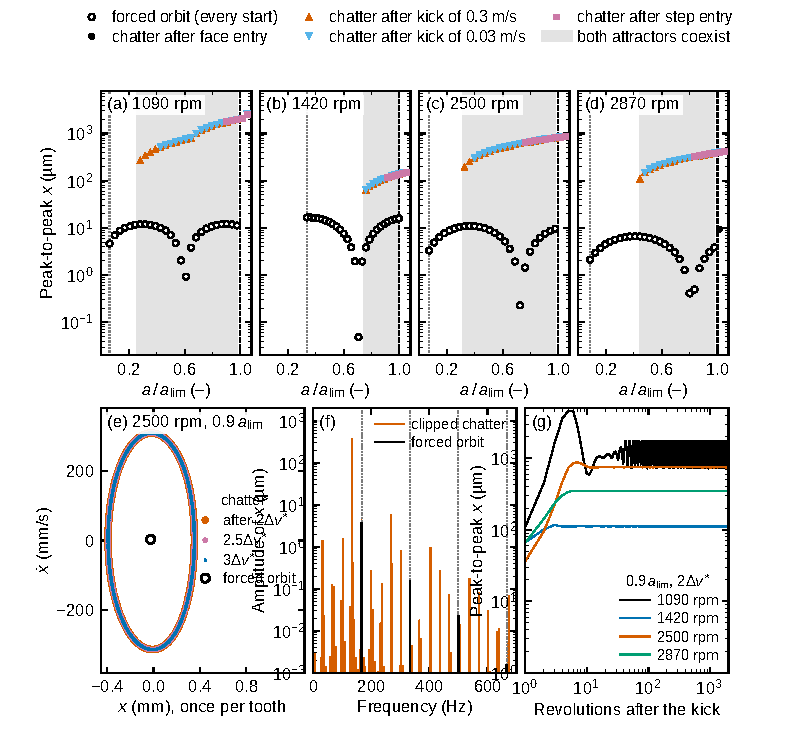
\includegraphics[width=\textwidth]{figures/fig_attractors.pdf}
  \caption{What lies beyond the basin ($g=\SI{1500}{\volt\second\per\metre}$, $\lvert V\rvert\le\SI{9}{\volt}$, full surface memory). (a)--(d)~Steady peak-to-peak displacement over the last 300 of 1600 revolutions against $a/\alim$, for four starts: open circles, the forced orbit, which every start reaches where it is the only attractor; filled markers, bounded chatter. Shaded: both attractors coexist; dotted: $\alim(0)$; dashed: $\alim$. (e)~Once-per-tooth samples of $(x,\dot x)$ of the last 500 tooth periods after kicks of 2, 2.5 and 3 times the critical kick, at \SI{2500}{\rpm} and $0.9\alim$: the three runs settle on the same closed curve around the forced orbit. (f)~Amplitude spectra of $x$ over 500 revolutions at the same point; dotted: tooth-passing harmonics. (g)~Peak-to-peak displacement per revolution after a kick of twice the critical kick at $0.9\alim$.}
  \label{fig:attr}
\end{figure}

\subsection{Describing-function prediction: further remarks}\label{supp:std-bistab-df}

The size of the basin near the limit can be predicted with a dual-input describing function \citep{gelb1968describing} (Section~\ref{M-sec:bistab-df}); \citet{ozsoy2025frequency} predicted the saturation of the settled cut in the frequency domain from its forced response, which is the forced command of Section~\ref{M-sec:model-orbit} (Section~\ref{M-sec:model-second}); their model has no threshold amplitude for disturbances.
A kick $\Delta v$ excites the chatter mode with a velocity amplitude $p\,\Delta v$, where $p$ was fitted on the unclipped cut from the decay of its least-damped mode after a small kick (Section~\ref{supp:bistab-df}).
In Eq.~\eqref{M-eq:dfbasin}, the limit holds because $g_e\to g$ and $\mathcal N(A)=1$ as long as $\bmax+A\le\Vmax$.
% src: src/c1_unsafe_zone.py (df_gain: 128 phases, b on 128 samples per tooth period; critical_amplitude; effective_gain_needed; _mode_factor: kick of 1 mm/s at phase 0, high-pass 40 Hz, fit of the slowest decaying mode)

Where $p$ could be fitted, from 0.7--$0.8\alim$ upwards, the simulated critical kick (median over the phases) is 0.61--1.13 times this estimate, and 0.88--1.13 times at 0.95 and $0.98\alim$ (Fig.~\ref{M-fig:basin}). Equation~\eqref{M-eq:dfbasin} predicts, without proving it, that the basin does not close at the limit but tends to a finite size set by the residual authority $\Vmax-\bmax$, which at $\alim$ is 3.9, 1.7, 0.87 and \SI{4.7}{\volt} at 1090, 1420, 2500 and \SI{2870}{\rpm}; at $0.999\alim$ the simulated critical kick is still 1.4--\SI{10.5}{\milli\metre\per\second} at the three speeds tested (Section~\ref{supp:bistab-basin}). The basin would close below $\alim$ only where $\bmax$ reached $\Vmax$, as it does at some depth below $\kappa\alim$ at the 94 speeds (1530--\SI{2460}{\rpm}) where the steady demand of Section~\ref{M-sec:feasibility} binds; persistent forcing that adds to $b$, such as runout, consumes the residual authority (Section~\ref{M-sec:delayed-robust}). The estimate is cheap, but it rests on the filtering hypothesis and on the factor $p$, fitted at one kick phase and valid only near the limit; $A^*$ is the harmonic-balance amplitude of the unstable limit cycle that bounds the basin.
% src: results/c1_df.npz (A_dual at a = a_lim: 3.92, 1.66, 0.87, 4.69 V at 1090, 1420, 2500, 2870 rpm = V_max - b_max; the 1420 rpm value was 0.009 V before a round-off fix in c1_unsafe_zone.critical_amplitude, tests/test_c1_results.py), results/c1_basin.npz (p_mode finite at frac >= 0.7, at 1420 rpm >= 0.8), results/c1_summary.json (td_over_df 0.61-1.13); ratios at 0.95/0.98 recomputed with the c1_summary formula: 0.88-1.13; verification/tdsim/check11_kick_near_limit.json (1.405-1.467, 7.055-7.611, 9.150-10.533 mm/s); README §11.5; verification/paper/revision_runs.json (closed_form.runout_to_clip_g1500: 0.730, 3.09, 8.74 um at 2500, 2870, 1420 rpm; 1090 rpm below 9 V up to 10 um; worst command over 40 depths up to 0.9 a_lim and 8 runout phases, c4_robust.worst_orbit_command)

\subsection{Checks of the protocols: summary}\label{supp:std-bistab-checks}

The protocols of Section~\ref{M-sec:bistability} were checked against their weak points (Section~\ref{supp:bistab-checks}). At $0.98\,\alim$, kicking at revolution 300 instead of 100 changes the critical kick at one of four phases per speed, by \SI{1.1}{\percent} (one bisection step), and the minimum over these phases at none; judging over 900 instead of 300 revolutions after the kick and using 64 instead of 16 kick phases change the worst-phase critical kick at the four speeds by at most \SI{1.1}{\percent}; the face entry leaves at revolution 100 a deviation from the forced orbit three orders of magnitude below the smallest critical kick. A scan of the band in steps of $0.05\,\alim$ at nine speeds, with the kicks of the band map, finds the lowest chattering depth next to the bisected edge at all nine and no chatter below it. At eight speeds the chattering depths form one interval up to $0.98\,\alim$; at \SI{520}{\rpm} they do not: kicks end in chatter at 0.30--$0.55\,\alim$ and at 0.95--$0.98\,\alim$, but at no grid depth in between. The mapped edge is therefore the lowest depth at which a kick of the protocol tips the cut, and the band above it need not be unsafe throughout.
% src: verification/paper/protocol_phases.json (summary: n_phases_available 64 at all four speeds; min over 64 phases against 16 at 0.98 a_lim: rel_change_of_min -0.0108 at 1090 rpm, 0 at 1420, 2500, 2870 rpm; all.largest_drop_of_min -0.0108); verification/paper/protocol_window.json (summary: 4 points, 53 runs, n_disagreeing_runs 0, ratio 1.0 at 1090/1420/2500/2870 rpm); verification/paper/protocol_kick_timing.json (units.residual_*: dev_x_from_orbit_um at rev100 <= 0.00085, dev_v_from_orbit_mmps <= 0.00073; summary.all: 16 points, ratio 0.989-1, max_abs_rel_change 0.0108; per speed ratio_of_minima 1.0; reproduction_all_identical true); verification/paper/protocol_band_holes.json (summary.all: speeds_complete 9, speeds_with_holes [520], speeds_with_chatter_below_edge [], total_runs 2028; summary.520: chatter_fracs 0.30-0.55, 0.95, 0.98, holes_above_edge 0.60-0.90; grid_edge_frac next to stored_edge_frac at all nine speeds)
